\chapter{2D Multi-view Incremental Decremental Discriminant Analysis}
\label{ch:2DMvIDDA}
\noindent {\textbf{\huge I}}n this chapter, we present an incremental-decremental classification method for 2D multi-view data. This method is based on 2DMvDA and extends it further by enabling the incremental learning and decremental unlearning of the data samples. It has similar formulations for incremental learning as that of MvIDA. However, it presents a decremental unlearning formulation as well.

This method, 2D Multi-view Incremental Decremental Discriminant Analysis (2DMvIDDA) supports the addition or deletion of data samples without retraining the model from scratch. Like MvIDA, this method also supports the addition of data samples from existing as well as previously unseen classes. Though the incremental formulations of 2DMvIDDA have been presented as one generalized case, they can be converted into the four specialized cases as those of MvIDA. Fig. \ref{fig:2DMvIDDA_Intro} shows an example of incremental learning and decremental unlearning of views.


\begin{figure}[t]
\centering
	\begin{subfigure}[t]{0.45\textwidth}
		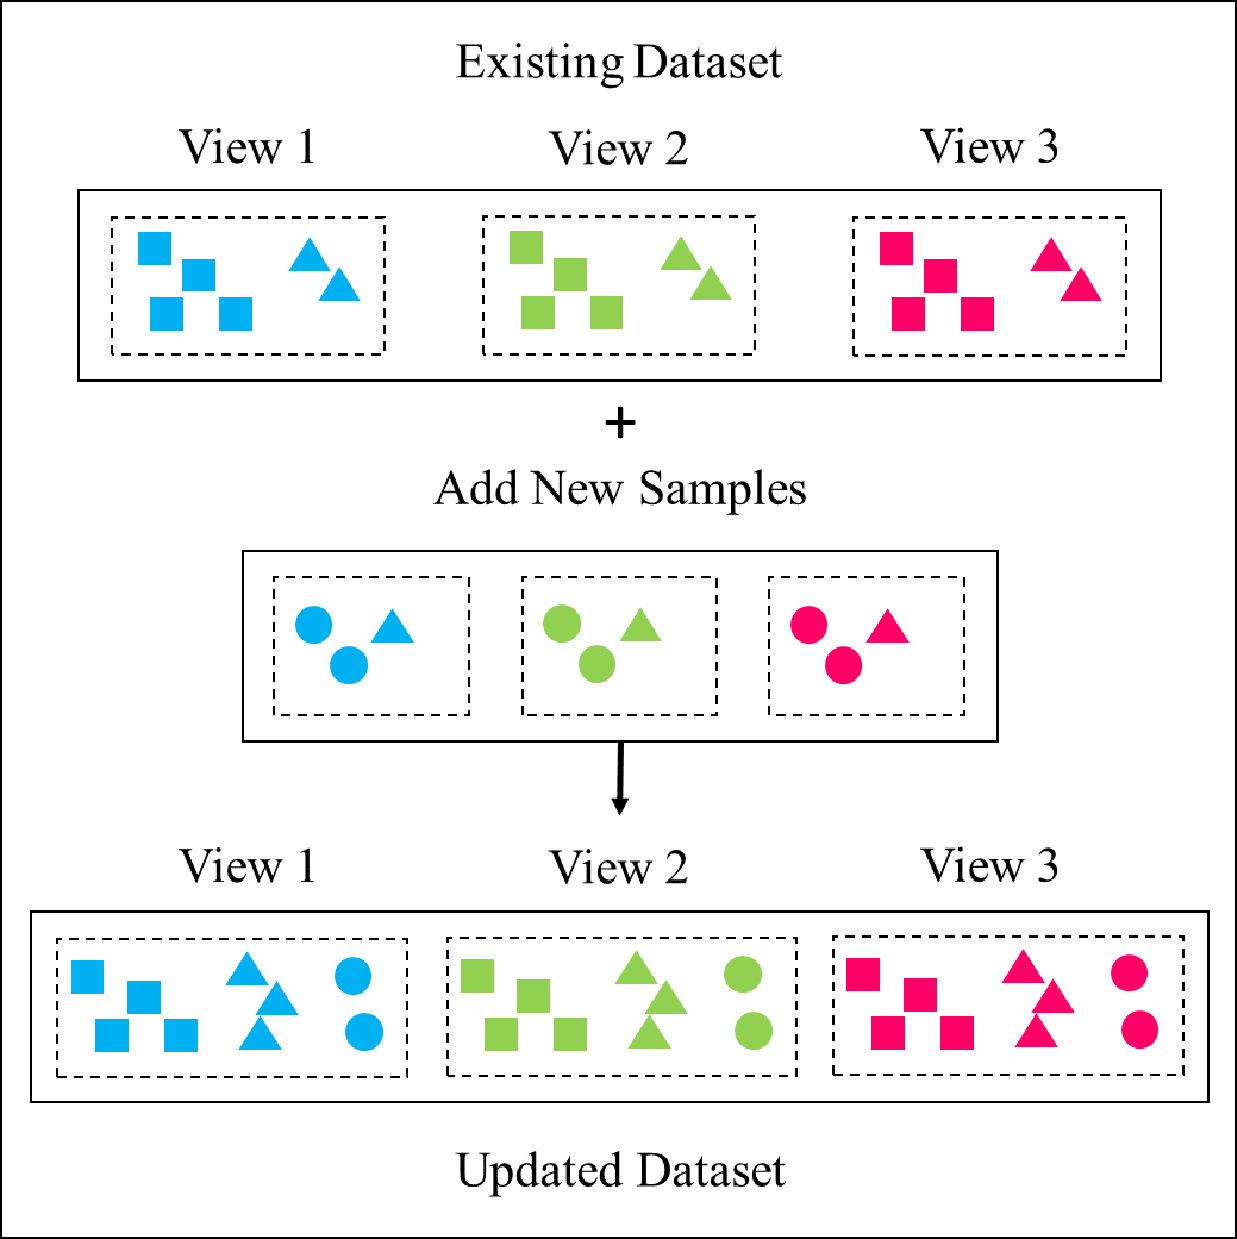
\includegraphics[width=\textwidth]{Figures/2DMvIDDA/Fig1.pdf}
		\caption{Incremental learning}
		\label{fig:2DMvIDDA_Intro_Inc}
	\end{subfigure}\hspace{0.2cm}
	\begin{subfigure}[t]{0.45\textwidth}
		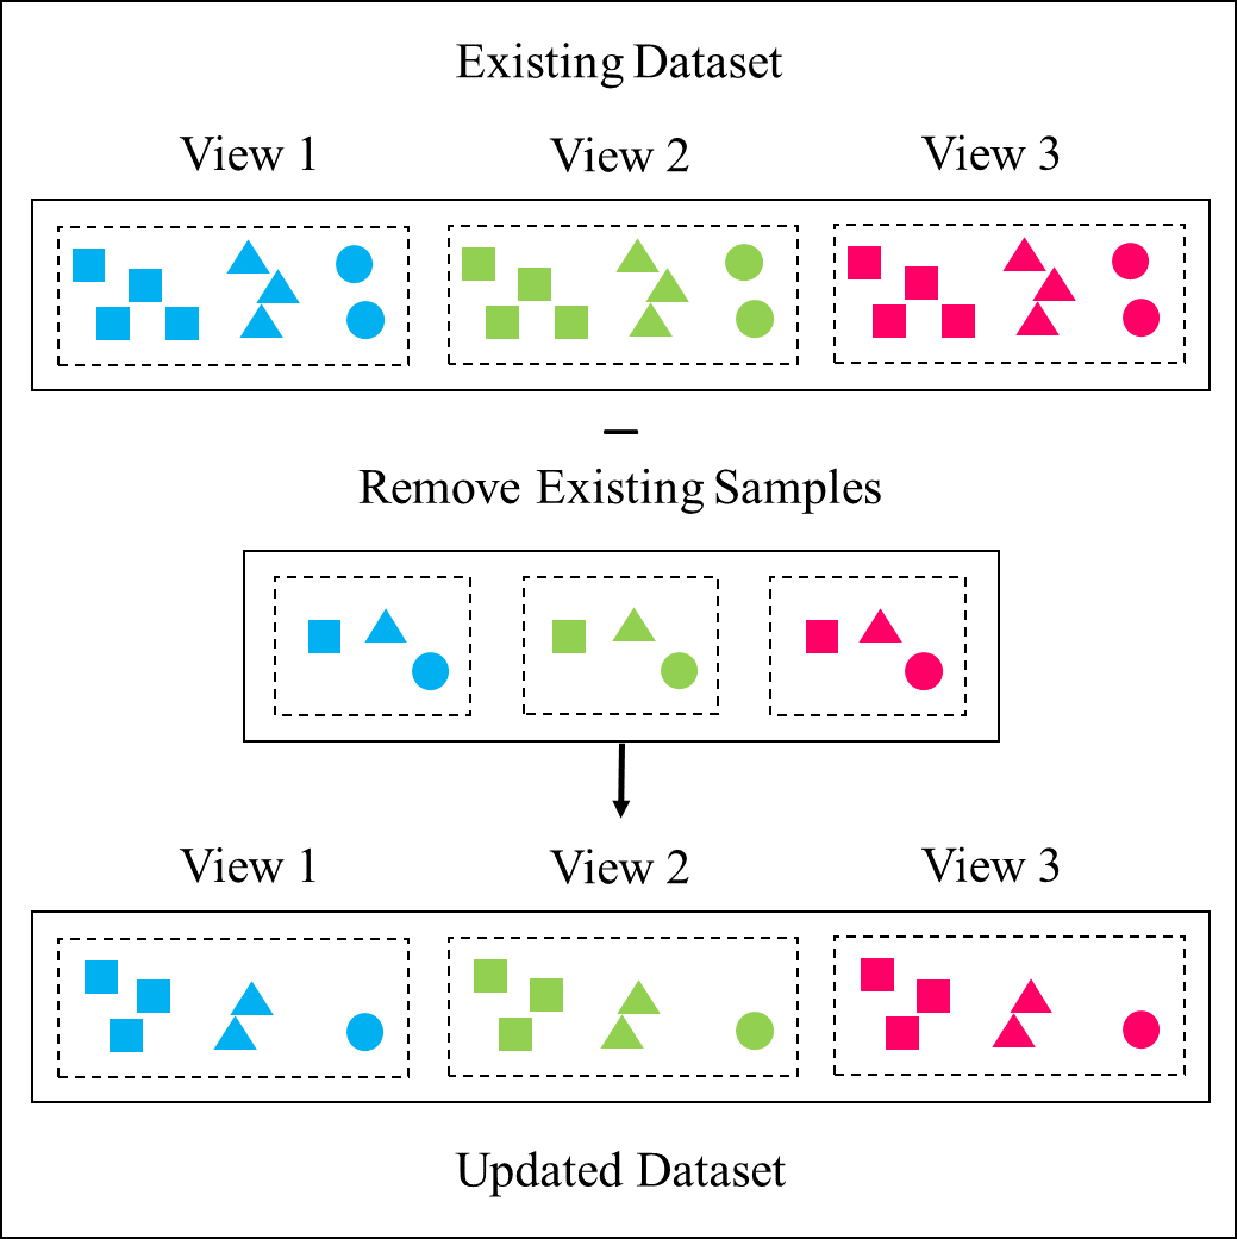
\includegraphics[width=\textwidth]{Figures/2DMvIDDA/Fig2.pdf}
		\caption{Decremental unlearning}
		\label{fig:2DMvIDDA_Intro_Dec}
	\end{subfigure}
\caption{Chunk increment and decrement : (a) A chunk of new data samples is added. Some of the new data samples belong to a new class. (b) A chunk of existing data samples is deleted from the dataset. Views are depicted with different colors (blue, green and red) and classes are depicted with different shapes (square, triangle and circle).}
\label{fig:2DMvIDDA_Intro}
\end{figure}

We present the formulations of 2DMvIDDA, the experimental setup, and results. We conclude this chapter by summarizing the features of the proposed method.



\section{Methodology}
\label{sec:2DMvIDDA_Algo}
\subsection{Addition of Data Samples}
\label{subs:2DMvIDDA_Inc}
Here, we present the update formulations for increments when a set of new data samples ($\bar{\mathcal{X}}$) is presented. The size of this set need not be the same for each increment. Some data samples in $\bar{\mathcal{X}}$ may belong to new classes. Let $\bar{\mathcal{Y}} = \{ \bar{\textbf{Y}}_{ijk} = \textbf{W}_j^T \bar{\textbf{X}}_{ijk} | i=1,\cdots,c'; j=1,\cdots,v; k=1,\cdots,\bar{n}_{ij} \}$ be the new set $\bar{\mathcal{X}}$ projected onto the shared subspace.

We then update the \textit{data sample counts} and the \textit{means} to include the new samples as follows:



\subsubsection{Updating the data sample counts}
\label{ssubs:2DMvIDDA_Inc_n}
The number of data samples per class per view, the number of data samples per class, and the total number of data samples are updated to include all the new data samples.

\begin{equation}
\label{eqn:nI}
n'_{ij} = n_{ij} + \bar{n}_{ij}, \hspace{0.2cm} n'_i = n_i + \bar{n}_i \hspace{0.2cm} \text{and} \hspace{0.2cm} n' = n + \bar{n}
\end{equation}

for $i = 1, \cdots, c'$ and $j = 1, \cdots, v$.



\subsubsection{Updating the means}
\label{ssubs:2DMvIDDA_Inc_M}
We update all the older means to reflect the change due to the addition of new data samples. The update equations are as follows-

\begin{equation}
\label{eqn:MijI}
{\textbf{M}_{ij}'}^{(\textbf{X})} = \frac{n_{ij} {\textbf{M}_{ij}}^{(\textbf{X})} + \sum\limits_{k=1}^{\bar{n}_{ij}} \bar{\textbf{X}}_{ijk}}{n_{ij} + \bar{n}_{ij}} = \frac{ n_{ij} {\textbf{M}_{ij}}^{(\textbf{X})} + \bar{n}_{ij} {\bar{\textbf{M}}_{ij}}^{(\textbf{X})}} {n_{ij}'}
\end{equation}
\begin{equation}
\label{eqn:MiI}
\textbf{M}'_{i} = \frac{n_i \textbf{M}_{i} + \sum\limits_{j=1}^{v} \sum\limits_{k=1}^{\bar{n}_{ij}} \bar{\textbf{Y}}_{ijk}}{n_i + \bar{n}_i} = \frac{n_i \textbf{M}_{i} + \bar{n}_i\bar{\textbf{M}}_{i}}{n_i'}
\end{equation}
\begin{equation}
\label{eqn:MI}
\textbf{M}' = \frac{n \textbf{M} + \sum\limits_{i=1}^{c'} \sum\limits_{j=1}^{v} \sum\limits_{k=1}^{\bar{n}_{ij}} \bar{\textbf{Y}}_{ijk}}{n+\bar{n}} = \frac{n \textbf{M} + \bar{n} \bar{\textbf{M}}}{n'}
\end{equation}

We then update the within-class and the between-class scatter matrix. Here, the equations are presented in the projected space first. Then, these equations are presented in terms of the original data samples for computation.




\subsubsection{Updating the within-class scatter matrix}
\label{ssubs:2DMvIDDA_Inc_Sw}
We only need to update the scatter of those classes to which new data samples are introduced. Hence, we have,
\small
\begin{equation}
\label{eqn:SwI}
\begin{split}
\textbf{S}_W' = & \sum\limits_{i \in \mathcal{UC}} \textbf{S}_{W_i} + \sum\limits_{i \in \mathcal{CH}} \sum\limits_{j=1}^{v} \sum\limits_{k=1}^{n_{ij}} \left( \textbf{Y}_{ijk} - \textbf{M}_i' \right) \left( \textbf{Y}_{ijk} - \textbf{M}_i' \right)^T + \sum\limits_{i \in \mathcal{CH}} \sum\limits_{j=1}^{v} \sum\limits_{k=1}^{\bar{n}_{ij}} \left( \bar{\textbf{Y}}_{ijk} - \textbf{M}_i' \right) \left( \bar{\textbf{Y}}_{ijk} - \textbf{M}_i' \right)^T \\
= & \sum\limits_{j=1}^{v} \sum\limits_{r=1}^{v} \textbf{W}_j^T \textbf{S}'_{jr} \textbf{W}_r
\end{split}
\end{equation}
\normalsize
where,
\small
\begin{equation}
\label{eqn:SjrI}
\begin{split}
\textbf{S}_{jr}' = \left\{\begin{matrix*}[l]
\textbf{S}_{jj} + \sum\limits_{i=1}^{c'} \bigg[ \frac{1}{\bar{n}_i n_i (n_i + \bar{n}_i)} \textbf{E} \textbf{E}^T - \frac{\bar{n}_{ij} \bar{n}_{ij}}{\bar{n}_i} \bar{\textbf{M}}_{ij}^{(\textbf{X})} \bar{\textbf{M}}_{ij}^{(A)^T} + \sum\limits_{k=1}^{\bar{n}_{ij}} \bar{\textbf{X}}_{ijk} \bar{\textbf{X}}_{ijk}^T \bigg] & j=r \\[0.3cm]
\textbf{S}_{jr} + \sum\limits_{i=1}^{c'} \bigg[ \frac{1}{\bar{n}_i n_i (n_i + \bar{n}_i)} \textbf{E} \textbf{F}^T - \frac{\bar{n}_{ij} \bar{n}_{ir}}{\bar{n}_i} \bar{\textbf{M}}_{ij}^{(\textbf{X})} \bar{\textbf{M}}_{ir}^{(A)^T} \bigg] & j \neq r
\end{matrix*}\right.
\end{split}
\end{equation}

\normalsize\noindent
here, \small$\textbf{E} = \bar{n}_{ij} n_i \bar{\textbf{M}}_{ij}^{(\textbf{X})} - \bar{n}_i n_{ij} \textbf{M}_{ij}^{(\textbf{X})}$ and $\textbf{F} = \bar{n}_{ir} n_i \bar{\textbf{M}}_{ir}^{(\textbf{X})} - \bar{n}_i n_{ir} \textbf{M}_{ir}^{(\textbf{X})}$.

The derivation of $\textbf{S}_{W}'$ and $\textbf{S}_{jr}'$ is given in Appendix-F%\ref{proof:2DMvIDDA_Sjr}
. Each submatrix of $S'$ consists of known quantities and is in closed form. This is true for the decremental formulation as well.


\begin{algorithm}[t]
\caption{2DMvIDDA: Incremental algorithm}
    \begin{algorithmic}
	\STATE \textbf{Input :}
	\STATE - A trained model $\phi$ that consists of:
	\STATE 		\hspace{0.3cm} - Data sample counts: $n$, $n_i$, $n_{ij}$
	\STATE 		\hspace{0.3cm} - Mean per class per view: $\textbf{M}_{ij}^{(\textbf{X})}$
	\STATE 		\hspace{0.3cm} - Scatter matrices: $\textbf{S}_{jr}$, $\textbf{D}_{jr}$
	\STATE 		\hspace{0.3cm} - Set of class labels of existing data samples: $\mathcal{C}$
	\STATE 		- Set of new data samples: $\bar{\mathcal{X}}$
	\STATE 		- Data sample counts of new data samples: $\bar{n}$, $\bar{n}_{i}$, $\bar{n}_{ij}$
	\STATE 		- Set of class labels of new data samples: $\bar{\mathcal{C}}$ \vspace{0.1cm}

	\WHILE{new data is encountered}
	
		\STATE \small Update $n$, $n_i$, $n_{ij}$ using Eq. (\ref{eqn:nI}).\;
		\STATE \small Update $\textbf{M}_{ij}^{(\textbf{X})}$ using Eq.(\ref{eqn:MijI}).\;
		\STATE \small Update $\textbf{S}_{jr}$ using Eq.(\ref{eqn:SjrI}).\;
		\STATE \small Update $\textbf{D}_{jr}$ using Eq.(\ref{eqn:DjrI}).\; \vspace{0.1cm}
		\STATE $\mathcal{C} = \mathcal{C} \cup \bar{\mathcal{C}}$.\;

		\STATE \small Compute the projection matrix $\textbf{W}^{opt}$ using Eq.(\ref{eqn:Lit_MvDA_GEP}).\;
	\ENDWHILE
	\STATE \textbf{Output :}
	\STATE - Updated model $\phi$
	\STATE - The projection matrix $\textbf{W}^{opt}$

\end{algorithmic}
\label{2DMvIDDA_Algo_Inc}
\end{algorithm}




\subsubsection{Updating the between-class scatter matrix}
\label{ssubs:2DMvIDDA_Inc_Sb}
This matrix is computed using only the updated class-mean ($\textbf{M}_{i}'$) and the total mean ($\textbf{M}'$). Both the means are updated after each increment, hence the scatter matrix is updated as,

\begin{equation}
\label{eqn:SbI}
\textbf{S}_B' = \sum\limits_{i=1}^{c'} n_{i}' (\textbf{M}_{i}' - \textbf{M}') (\textbf{M}_{i}' - \textbf{M}')^T = \sum\limits_{j=1}^{v} \sum\limits_{r=1}^{v} \textbf{W}_j^T \textbf{D}'_{jr} \textbf{W}_r
\end{equation}
where each $\textbf{D}_{jr}$ is given as,
\begin{equation}
\label{eqn:DjrI}
\begin{split}
\textbf{D}_{jr}' = & \; \sum\limits_{i=1}^{c'} \; \frac{n_{ij}' \; n_{ir}'}{n_{i}'} \; {\textbf{M}_{ij}'}^{(\textbf{X})} {{\textbf{M}_{ir}'}^{(\textbf{X})}}^T - \frac{1}{n'} \left (\sum\limits_{i=1}^{c'} n_{ij}' \; {\textbf{M}_{ij}'}^{(\textbf{X})} \right ) \left (\sum\limits_{i=1}^{c'} n_{ir}' \; {{\textbf{M}_{ir}'}^{(\textbf{X})}} \right )^T
\end{split}
\end{equation}

\noindent
The derivation of $\textbf{S}_{B}'$ and $\textbf{D}_{jr}'$ is given in Appendix-A.%\ref{proof:Djr}.

After updating the means and the scatter matrices, 2DMvIDDA computes the optimal projection matrix $\textbf{W}^{opt}$ using Eq. \ref{eqn:Lit_MvDA_GEP}. The test data samples can be classified using this projection matrix until new training data samples are presented, or any of the existing ones are deleted. If new data samples are added, these steps are repeated. The incremental learning formulation is summarized in Algorithm\ref{2DMvIDDA_Algo_Inc}.




\subsection{Deletion of Data Samples}
\label{subs:2DMvIDDA_Dec}
Here, we present the update formulations for decremental unlearning when a subset ($\bar{\mathcal{X}}$) of existing data samples is to be deleted. $\bar{\mathcal{X}}$ may have one or more data samples in it. The projection of $\bar{\mathcal{X}}$ onto the shared subspace is given as $\bar{\mathcal{Y}} = \{ \bar{\textbf{Y}}_{ijk} = \textbf{W}_j^T \bar{\textbf{X}}_{ijk} | i=1, \cdots ,c; j=1, \cdots ,v; k=1, \cdots ,\bar{n}_{ij} \}$.

We update the \textit{data sample counts} and the \textit{means} to reflect the changes in the dataset after the decrement.



\subsubsection{Updating the data sample counts}
\label{ssubs:2DMvIDDA_Inc_n}
The number of data samples per class per view, number of data samples per class, and the total number of data samples are updated to reflect the deletion of the data samples in $\bar{\mathcal{X}}$.

\begin{equation}
\label{eqn:n_Dec}
n'_{ij} = n_{ij} - \bar{n}_{ij}, \hspace{0.2cm} n'_i = n_i - \bar{n}_i \hspace{0.2cm} \text{and} \hspace{0.2cm} n' = n - \bar{n}
\end{equation}

for $i = 1, \cdots, c$ and $j = 1, \cdots, v$.



\subsubsection{Updating the means}
\label{ssubs:2DMvIDDA_Inc_M}
We update all the older means to reflect the change due to the deletion of new data samples. The update equations are as follows-

\begin{equation}
\label{eqn:Mij_Dec}
{\textbf{M}_{ij}'}^{(\textbf{X})} = \frac{n_{ij} {\textbf{M}_{ij}}^{(\textbf{X})} - \sum\limits_{k=1}^{\bar{n}_{ij}} \bar{\textbf{X}}_{ijk}}{n_{ij} - \bar{n}_{ij}} = \frac{ n_{ij} {\textbf{M}_{ij}}^{(\textbf{X})} - \bar{n}_{ij} {\bar{\textbf{M}}_{ij}}^{(\textbf{X})}} {n_{ij}'}
\end{equation}
\begin{equation}
\label{eqn:Mi_Dec}
\textbf{M}'_{i} = \frac{n_i \textbf{M}_{i} - \sum\limits_{j=1}^{v} \sum\limits_{k=1}^{\bar{n}_{ij}} \bar{\textbf{Y}}_{ijk}}{n_i - \bar{n}_i} = \frac{n_i \textbf{M}_{i} - \bar{n}_i\bar{\textbf{M}}_{i}}{n_i'} \end{equation}
\begin{equation}
\label{eqn:M_Dec}
\textbf{M}' = \frac{n \textbf{M} - \sum\limits_{i=1}^{c} \sum\limits_{j=1}^{v} \sum\limits_{k=1}^{\bar{n}_{ij}} \bar{\textbf{Y}}_{ijk}}{n-\bar{n}} = \frac{n \textbf{M} - \bar{n} \bar{\textbf{M}}}{n'}
\end{equation}



\begin{algorithm}[t]
\caption{2DMvIDDA: Decremental algorithm}
    \begin{algorithmic}
	\STATE \textbf{Input :}
	\STATE - A trained model $\phi$ that consists of:
	\STATE 		\hspace{0.3cm} - Data sample counts: $n$, $n_i$, $n_{ij}$
	\STATE 		\hspace{0.3cm} - Mean per class per view: $\textbf{M}_{ij}^{(\textbf{X})}$
	\STATE 		\hspace{0.3cm} - Scatter matrices: $\textbf{S}_{jr}$, $\textbf{D}_{jr}$
	\STATE 		\hspace{0.3cm} - Set of class labels of existing data samples: $\mathcal{C}$
	\STATE 		- Set of data samples to be deleted: $\bar{\mathcal{X}}$
	\STATE 		- Data sample counts of the samples to be deleted: $\bar{n}$, $\bar{n}_{i}$, $\bar{n}_{ij}$
	\STATE 		- Set of classes that are empty after deletion: $\hat{\mathcal{C}}$ \vspace{0.1cm}

	\WHILE{$\bar{\mathcal{X}}$ is not empty}
		\STATE \small Update $n$, $n_i$, $n_{ij}$ using Eq. (\ref{eqn:n_Dec}).\;
		\STATE \small Update $\textbf{M}_{ij}^{(\textbf{X})}$ using Eq.(\ref{eqn:Mij_Dec}).\;
		\STATE \small Update $\textbf{S}_{jr}$ using Eq.(\ref{eqn:Sjr_Dec}).\;
		\STATE \small Update $\textbf{D}_{jr}$ using Eq.(\ref{eqn:Djr_Dec}).\; \vspace{0.1cm}
		\STATE $\mathcal{C} = \mathcal{C} - \hat{\mathcal{C}}$.\;
		
		\STATE \small Compute the projection matrix $\textbf{W}^{opt}$ using Eq.(\ref{eqn:Lit_MvDA_GEP}).\;
	\ENDWHILE
	\STATE \textbf{Output :}
	\STATE - Updated model $\phi$
	\STATE - The projection matrix $\textbf{W}^{opt}$

\end{algorithmic}
\label{Algo_Dec}
\end{algorithm}



\subsubsection{Updating the within-class scatter matrix}
\label{ssubs:2DMvIDDA_Inc_Sw}
We only need to update the scatter of those classes from which some existing data samples are deleted. So, we have,

\small
\begin{equation}
\label{eqn:Sw_Dec}
\begin{split}
\textbf{S}_W' = & \sum\limits_{i \in \mathcal{UC}} \textbf{S}_{W_i} + \sum\limits_{i \in \mathcal{CH}} \sum\limits_{j=1}^{v} \sum\limits_{k=1}^{n_{ij}} \left( \textbf{Y}_{ijk} - \textbf{M}_i' \right) \left( \textbf{Y}_{ijk} - \textbf{M}_i' \right)^T - \sum\limits_{i \in \mathcal{CH}} \sum\limits_{j=1}^{v} \sum\limits_{k=1}^{\bar{n}_{ij}} \left( \bar{\textbf{Y}}_{ijk} - \textbf{M}_i' \right) \left( \bar{\textbf{Y}}_{ijk} - \textbf{M}_i' \right)^T \\
= & \sum\limits_{j=1}^{v} \sum\limits_{r=1}^{v} \textbf{W}_j^T \textbf{S}'_{jr} \textbf{W}_r
\end{split}
\end{equation}
where,
\begin{equation}
\label{eqn:Sjr_Dec}
\begin{split}
\textbf{S}_{jr}' = \left\{\begin{matrix*}[l]
\textbf{S}_{jj} - \sum\limits_{i \in \mathcal{CH}} \bigg[ \frac{1}{\bar{n}_i n_i (n_i - \bar{n}_i)} \textbf{E} \textbf{E}^T - \frac{\bar{n}_{ij} \bar{n}_{ij}}{\bar{n}_i} \bar{\textbf{M}}_{ij}^{(\textbf{X})} \bar{\textbf{M}}_{ij}^{(A)^T} - \sum\limits_{k=1}^{\bar{n}_{ij}} \bar{\textbf{X}}_{ijk} \bar{\textbf{X}}_{ijk}^T \bigg] & j=r \\[0.3cm]
\textbf{S}_{jr} - \sum\limits_{i \in \mathcal{CH}} \bigg[ \frac{1}{\bar{n}_i n_i (n_i - \bar{n}_i)} \textbf{E} \textbf{F}^T + \frac{\bar{n}_{ij} \bar{n}_{ir}}{\bar{n}_i} \bar{\textbf{M}}_{ij}^{(\textbf{X})} \bar{\textbf{M}}_{ir}^{(A)^T} \bigg] & j \neq r
\end{matrix*}\right.
\end{split}
\end{equation}

\noindent
here, \small$\textbf{E} = \bar{n}_{i} n_{ij} \textbf{M}_{ij}^{(\textbf{X})} - \bar{n}_{ij} n_{i} \bar{\textbf{M}}_{ij}^{(\textbf{X})}$ and $\textbf{F} = \bar{n}_{i} n_{ir} \textbf{M}_{ir}^{(\textbf{X})} - \bar{n}_{ir} n_{i} \bar{\textbf{M}_{ir}}^{(\textbf{X})}$. The derivation of $\textbf{S}_{W}'$ and $\textbf{S}_{jr}'$ is similar to that of incremental formulations given in Appendix-F %\ref{proof:2DMvIDDA_Sjr}
and hence is not presented separately.



\subsubsection{Updating the between-class scatter matrix}
\label{ssubs:2DMvIDDA_Inc_Sb}
The between-class scatter matrix is updated as,

\begin{equation}
\label{eqn:Sb_Dec}
\textbf{S}_B' = \sum\limits_{i=1}^{c'} n_{i}' (\textbf{M}_{i}' - \textbf{M}') (\textbf{M}_{i}' - \textbf{M}')^T = \sum\limits_{j=1}^{v} \sum\limits_{r=1}^{v} \textbf{W}_j^T \textbf{D}'_{jr} \textbf{W}_r
\end{equation}
where each $\textbf{D}_{jr}$ is given as,
\begin{equation}
\label{eqn:Djr_Dec}
\begin{split}
\textbf{D}_{jr}' = & \; \sum\limits_{i=1}^{c'} \; \frac{n_{ij}' \; n_{ir}'}{n_{i}'} \; {\textbf{M}_{ij}'}^{(\textbf{X})} {{\textbf{M}_{ir}'}^{(\textbf{X})}}^T - \frac{1}{n'} \left (\sum\limits_{i=1}^{c'} n_{ij}' \; {\textbf{M}_{ij}'}^{(\textbf{X})} \right ) \left (\sum\limits_{i=1}^{c'} n_{ir}' \; {{\textbf{M}_{ir}'}^{(\textbf{X})}} \right )^T
\end{split}
\end{equation}

The derivation of $\textbf{S}_{B}'$ and $\textbf{D}_{jr}'$ is as given in Appendix-A.%\ref{proof:Djr}.

After updating the means and the scatter matrices, we update $\mathcal{C}$ by removing the labels of classes from which all the data samples were deleted. 2DMvIDDA then computes the optimal projection matrix $\textbf{W}^{opt}$ using Eq. \ref{eqn:Lit_MvDA_GEP}. The test data samples can be classified using this projection matrix until new training data samples are added, or some existing ones are deleted. If any data samples are deleted, the model is updated using the aforementioned formulations. The formulations of decremental unlearning are presented in Algorithm \ref{Algo_Dec}.










\subsection{Discussion}
\label{subs:2DMvIDDA_Discussion}
In this section, we discuss how the discriminant methods, namely 2DMvDA, MvIDA, MvDA, 2DLDA, and ILDA, are special cases of the proposed method 2DMvIDDA. We also state how their formulations can be obtained from 2DMvIDDA formulations.



\subsubsection{2D Multi-view Discriminant Analysis (2DMvDA)}
\label{ssubs:2DMvIDDA_2DMvDA}
2DMvDA is a discriminant analysis-based method for 2D Multi-view data. Let $\mathcal{A} = \{ \textbf{A}_{ijk} | i=1,\cdots,c; j=1,\cdots,v; k=1,\cdots,n_{ij} \}$ be the training set for 2DMvDA. Each $\textbf{A}_{ijk} \in \mathbb{R}^{p_j \times q}$. The incremental formulation of 2DMvIDDA can be used as 2DMvDA by treating all the data samples as a new set having data samples from $c$ new classes. Here, the existing samples will be $0$ as no data samples were already presented for training. Once the scatter matrices are computed using these formulations, the projection matrix $\textbf{W}^{opt}$ can be obtained by using Eq. \ref{eqn:Lit_MvDA_GEP}.




\subsubsection{Multi-view Incremental Discriminant Analysis (MvIDA)}
\label{ssubs:2DMvIDDA_MvIDA}
MvIDA is a discriminant analysis-based incremental method for 1D multi-view data. Let the dataset be denoted as $\mathcal{A} = \{ \textbf{a}_{ijk} | i=1,\cdots,c; j=1,\cdots,v; k=1,\cdots,n_{ij} \}$. Each $\textbf{a}_{ijk} \in \mathbb{R}^{1 \times q}$. The incremental learning formulations of 2DMvIDDA can be used as MvIDA if we keep the number of rows ($p_j$) of every data sample equal to $1$, as MvIDA takes 1D data samples as input. The four incremental formulations of MvIDA are just the special cases of the incremental formulation of 2DMvIDDA. Hence, once the scatter matrices are computed using the incremental formulations according to the type of increment, the projection matrix $\textbf{W}^{opt}$ can be obtained by using Eq. \ref{eqn:Lit_MvDA_GEP}. We can also extend MvIDA to include the decremental unlearning using the decremental formulations of 2DMvIDDA.




\subsubsection{Multi-view Discriminant Analysis (MvDA)}
\label{ssubs:2DMvIDDA_MvDA}
MvDA is a discriminant analysis-based batch method for 1D multi-view data. Let the dataset be denoted as $\mathcal{A} = \{ \textbf{a}_{ijk} | i=1,\cdots,c; j=1,\cdots,v; k=1,\cdots,n_{ij} \}$. Each $\textbf{a}_{ijk} \in \mathbb{R}^{1 \times q}$. The incremental formulation of 2DMvIDDA can be used as MvDA by 
\begin{itemize}
	\item Keeping the number of rows ($p_j$) of every data sample equal to $1$, as MvDA takes 1D data samples as input.
	\item Treating all the data samples as one set of data having data samples from $c$ new classes.
\end{itemize}
Here, the existing samples will be $0$ as no data samples were already presented to the model. Once the scatter matrices are computed using these formulations of 2DMvIDDA, the projection matrix $\textbf{W}^{opt}$ is obtained using Eq.\ref{eqn:Lit_MvDA_GEP}.




\subsubsection{2D Linear Discriminant Analysis (2DLDA)}
\label{ssubs:2DMvIDDA_2DLDA}
2DLDA is a discriminant analysis-based batch method that trains on the single-view 2D data. Let $\mathcal{A} = \{ \textbf{A}_{ijk} | i=1,\cdots,c; j=1; k=1,\cdots,n_{ij} \}$ be the whole training set for 2DLDA. Each $\textbf{A}_{ijk} \in \mathbb{R}^{p \times q}$ and $j = 1$ as there is only one view. The incremental formulation of 2DMvIDDA can be used as 2DLDA by treating all the data samples as the set of new data having data samples from $c$ new classes and only one view. The number of existing samples will be $0$ as no data samples were already presented to the model. The projection matrix $\textbf{W}^{opt}$ can be obtained by using Eq. \ref{eqn:Lit_MvDA_GEP} after the scatter matrices are computed using the incremental formulations of 2DMvIDDA.




\subsubsection{Incremental Linear Discriminant Analysis (ILDA)}
\label{ssubs:2DMvIDDA_ILDA}
ILDA is an incremental method based on discriminant analysis and trains on 1D single-view data. Let the dataset be denoted as $\mathcal{A} = \{ \textbf{a}_{ijk} | i=1,\cdots,c; j=1; k=1,\cdots,n_{ij} \}$. Each $\textbf{a}_{ijk} \in \mathbb{R}^{1 \times q}$. The incremental formulations of 2DMvIDDA can be used as ILDA by 
\begin{itemize}
	\item Keeping the number of rows ($p_j$) of every data sample equal to $1$, as ILDA takes 1D data samples as input.
	\item Keeping $j = 1$ as ILDA is a single-view method.
\end{itemize}
The optimal projection matrix $\textbf{W}^{opt}$ can be obtained by using Eq. \ref{eqn:Lit_MvDA_GEP} after the scatter matrices are computed using the suitable formulations according to the type of increment. Similar to the incremental formulations, we can also formulate a decremental version of ILDA using the decremental formulations of 2DMvIDDA.












\section{Experiments and Results}
\label{sec:2DMvIDDA_Expt}

\subsection{Experimental Setup}
\label{subs:2DMvIDDA_Expt_Setup}
We divided the datasets into two parts: the training dataset has 80\% of the data samples, and the remaining (20\%) are used for testing. The training set is used to simulate increments and decrements in the data. We have taken sets of 20 data samples for each increment or decrement.

The experiments that compare all the 2D and 1D methods are performed using rescaled versions of the datasets owing to the greater memory needs of 1D methods. We compare the classification accuracy, training time, and memory requirements of 2DMvIDDA to the methods discussed in Section \ref{subs:2DMvIDDA_Discussion}.

The experiments that compare only the 2D methods are performed on the original datasets to show that the 2D methods require much less time and memory, even for large images. Here, the classification accuracy remains the same as when the rescaled versions were used. Hence, we focus on the training time and memory requirements. The methodology for classification is the same as that used for MvIDA.





\subsection{Results}
\label{subs:2DMvIDDA_Res}
This section presents the results of experiments designed in order to answer the research questions posed in chapter \ref{ch:Intro}. Research question 1 and 2 are answered in sections \ref{ssubs:2DMvIDDA_Subspace} and \ref{ssubs:2DMvIDDA_OI}. The third question is answered in two parts in sections \ref{ssubs:2DMvIDDA_Rescaled} and \ref{ssubs:2DMvIDDA_Orig}.

\subsubsection{Similarity of the Discriminant Subspace}
\label{ssubs:2DMvIDDA_Subspace}
\begin{itemize}
\item \textbf{RQ1 :}
Can the 2D incremental-decremental method, without using old data samples, produce an identical model to that of its batch counterpart, 2DMvDA?

\item \textbf{Experiment :}
To compare the discriminant subspace, we incrementally trained two models using 2DMvIDDA and 2DMvDA, respectively. Then, we deleted existing data samples from the dataset in a similar fashion. At each update, the inner products of the first five eigenvectors of both models are computed. As the eigenvectors are of unit length, we say two eigenvectors are equal when their inner product is 1.

\item \textbf{Discussion :}
Fig. \ref{fig:2DMvIDDA_Res_Subspace} presents the inner products computed over the updates on the Stereo Face dataset. The inner products are presented for the increments from $0$ to $640$ data samples at first. Then, the inner products for the decrements from $640$ to $0$ data samples are shown. The figure shows the inner products converged to $1$ for all updates, except for the first few increments and the last few sets of decrements. This implies that the shared discriminant subspace constructed by 2DMvIDDA is the same as that constructed by 2DMvDA. A minor difference is seen in the case of first few increments, as the less number of data samples causes some inaccuracies in eigenvalue computation. The same is observed at the end of decrements too.
\end{itemize}

\begin{figure}[t]
	\centering
    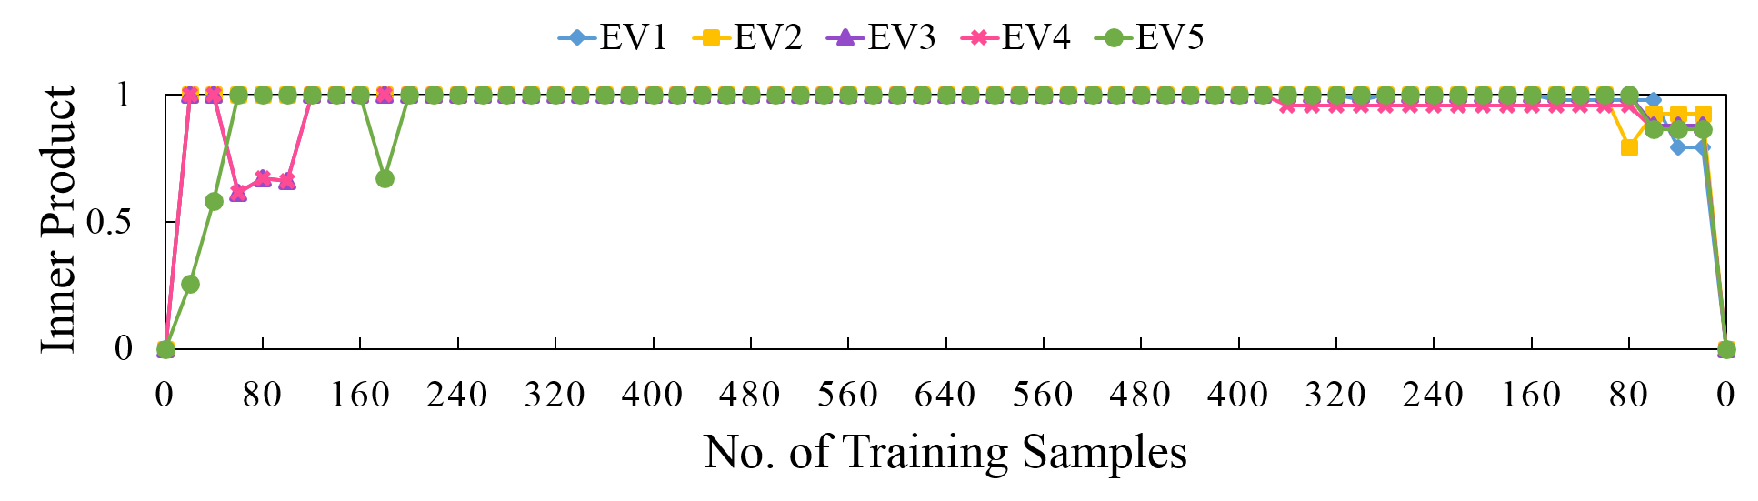
\includegraphics[width=\textwidth]{Figures/2DMvIDDA/Fig3.pdf}
	\caption{Inner product between first five eigenvectors of 2DMvIDDA and 2DMvDA for Stereo face dataset during incremental and decremental phases.}
	\label{fig:2DMvIDDA_Res_Subspace}
\end{figure}








\begin{figure}[t]
	\centering
	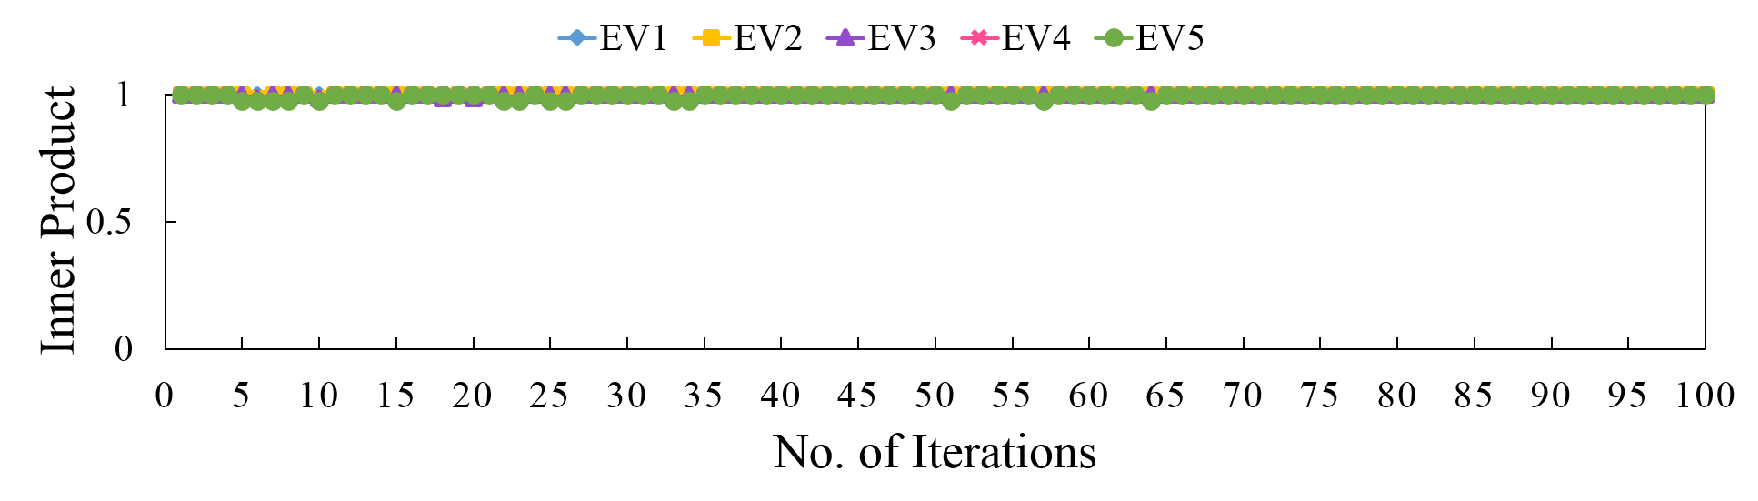
\includegraphics[width=\textwidth]{Figures/2DMvIDDA/Fig4.pdf}
	\caption{Inner product of the eigenvectors over 100 iterations of 2DMvIDDA with those of 2DMvDA.}
	\label{fig:2DMvIDDA_Res_OI}
\end{figure}

\subsubsection{Order Independence}
\label{ssubs:2DMvIDDA_OI}
\begin{itemize}
\item \textbf{RQ2 :}
Is this method invariant to the order of addition or deletion of data samples?

\item \textbf{Experiment :}
We trained the model using 2DMvIDDA on the training set a hundred times by adding or deleting the data samples in a randomized order every time. When updates are done after each iteration, we compute the inner product of eigenvectors of the trained model with the eigenvectors of the batch method, 2DMvDA.

\item \textbf{Discussion :}
We experimented on all four datasets and found that the inner product of eigenvectors from both models is equal to or very close to $1$ every time. To avoid redundancy, we only present the results for the Stereo Face dataset in Fig. \ref{fig:2DMvIDDA_Res_OI}. Here, we see the inner products of these eigenvectors are converged to $1$. This proves the order independence of the proposed method.
\end{itemize}





\subsubsection{Comparison on the Rescaled Datasets}
\label{ssubs:2DMvIDDA_Rescaled}

\begin{table}[t]
	\centering
	\caption{Comparison of 2DMvIDDA with other methods based on discriminant analysis}
	\label{tab:2DMvIDDA_Res_All_RS}
	\begin{tabular}{l l c r r} \hline
		
		 &  & \textbf{Classification} & \multicolumn{1}{c}{\textbf{Memory}} & \textbf{Training Time} \\
		\textbf{Dataset} & \textbf{Method} & \textbf{Accuracy (\%)} & \multicolumn{1}{c}{\textbf{(MBs)}} & \multicolumn{1}{c}{\textbf{(seconds)}} \\ \hline
		 
		       & \textbf{2DMvIDDA} & \textbf{100.00} & \textbf{3.24} & \textbf{0.11} \\ 
			   & 2DMvDA   & 100.00 & 13.60 & 0.15 \\ 
		IMPART & MvIDA    & 100.00 & 10751.61 & 587.31 \\ 
			   & MvDA     & 100.00 & 10761.98 & 1835.93 \\ 
			   & 2DLDA    & 100.00 & 13.60 & 1.32 \\ 
			   & ILDA     & - & - & - \\ \hline
	
			   & \textbf{2DMvIDDA} & \textbf{98.67} & \textbf{1.49} & \textbf{0.01} \\ 
			   & 2DMvDA   & 98.67 & 29.75 & 0.14 \\ 
	   MSSpoof & MvIDA    & 90.67 & 1678.95 & 647.63 \\ 
			   & MvDA     & 90.67 & 1707.21 & 2551.35 \\ 
			   & 2DLDA    & 96.00 & 29.75 & 1.54 \\ 
			   & ILDA     & 86.66 & 1677.72 & 3915.05 \\ \hline
	
			   & \textbf{2DMvIDDA} & \textbf{75.62} & \textbf{20.25} & \textbf{0.19} \\ 
			   & 2DMvDA   & 75.62 & 157.87 & 0.93 \\ 
		Stereo & MvIDA    & 73.75 & 9682.16 & 1423.10 \\ 
		Face   & MvDA     & 73.75 & 9811.52 & 3970.58 \\ 
			   & 2DLDA    & 75.00 & 157.87 & 12.24 \\ 
			   & ILDA     & 70.78 & 9663.67 & 90863.35 \\ \hline
	
			   & \textbf{2DMvIDDA} & \textbf{91.25} & \textbf{5.85} & \textbf{0.11} \\ 
			   & 2DMvDA   & 91.25 & 45.41 & 0.70 \\ 
		ORL    & MvIDA    & 81.25 & 1916.05 & 806.30 \\ 
			   & MvDA     & 81.25 & 1955.61 & 1777.62 \\ 
			   & 2DLDA    & 86.25 & 45.41 & 2.95 \\ 
			   & ILDA     & 57.50 & 1911.10 & 5561.28 \\ \hline
	\end{tabular}
\end{table}

\begin{itemize}
\item \textbf{RQ3 :}
How is this method more advantageous than other discriminant analysis-based methods?

\item \textbf{Experiment :}
We trained models using 2DMvIDDA, 2DMvDA, MvIDA, MvDA, 2DLDA, and ILDA on the rescaled versions of the datasets due to the memory constraints of 1D methods. However, ILDA could not run even on the rescaled version of IMPART dataset. Parameters for the rest of the methods on all the datasets have been recorded.

\item \textbf{Discussion :}
Table \ref{tab:2DMvIDDA_Res_All_RS} lists the parameters recorded for the above-mentioned methods. Here, we see that 2DMvIDDA shows the highest classification accuracy with the lowest time and memory requirements among all these methods.

The reason for the higher classification accuracy is the use of multiple views and the 2D form of the data. For the same reasons, 2DMvDA also has the same accuracy as 2DMvIDDA, but it takes much more time and memory for training. MvIDA and MvDA use the multi-view data effectively, but they lose the spatial information as they use a vectorized form of images. 2DLDA uses the 2D form of data, but it merges all the views and hence does not benefit from the contrasting information that each view offers. ILDA has the least classification accuracy as it uses neither the multiple views separately nor the 2D form of the data.

2DMvIDDA requires less memory than the rest because (i) the use of 2D form leads to smaller scatter matrices, and (ii) as it is an incremental method, it only needs to store the existing model and the data samples to be added or deleted. It does not need to store the whole dataset, unlike the batch


\begin{figure}[h]
\centering
  \begin{subfigure}[h]{0.45\textwidth}
    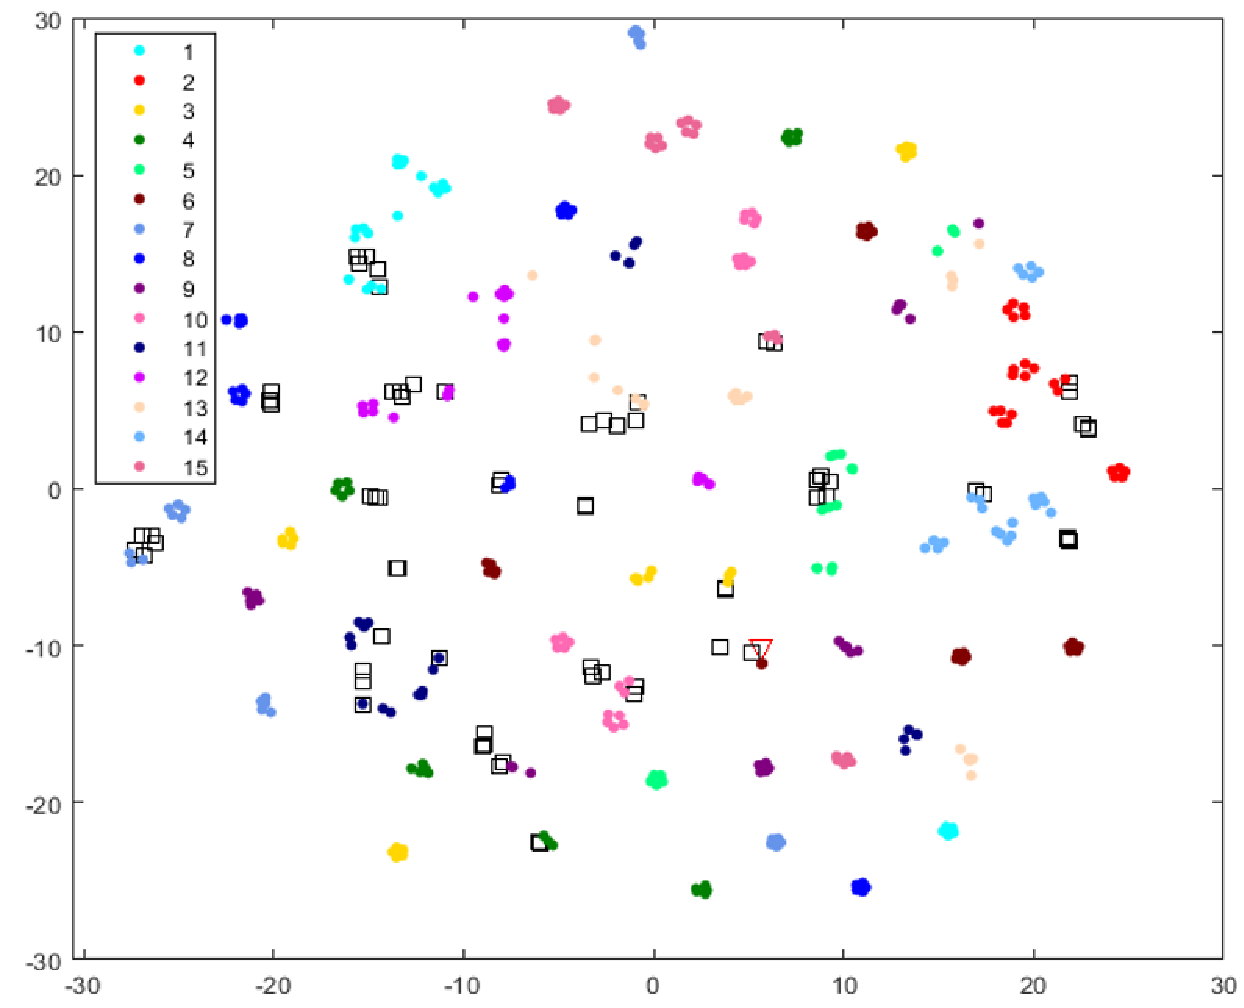
\includegraphics[width=\textwidth]{Figures/2DMvIDDA/Fig5.pdf}
    \caption{2DMvIDDA}
  \end{subfigure}
  \begin{subfigure}[h]{0.45\textwidth}
    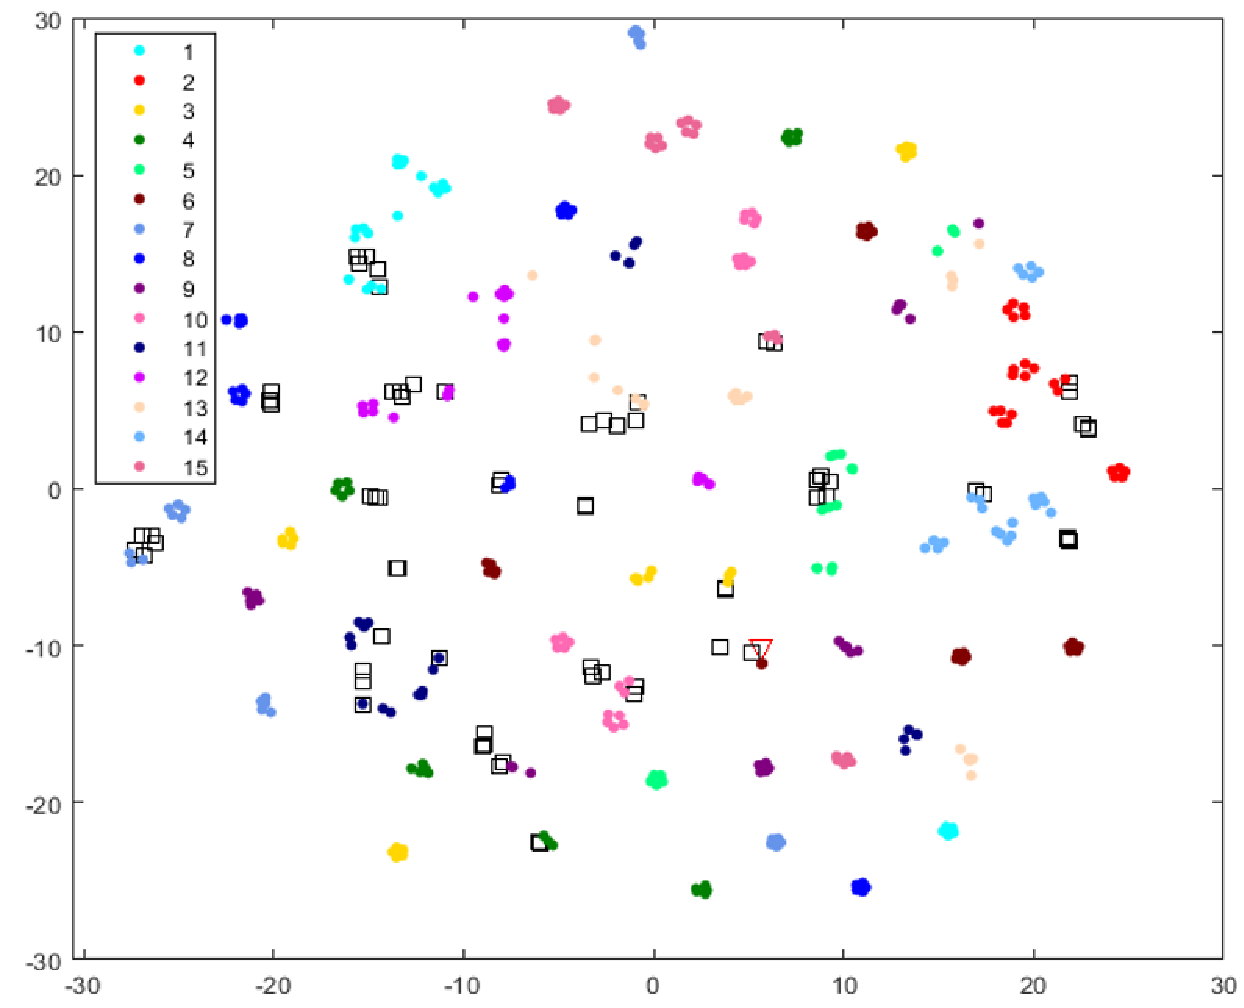
\includegraphics[width=\textwidth]{Figures/2DMvIDDA/Fig6.pdf}
    \caption{2DMvDA}
  \end{subfigure}

  \begin{subfigure}[h]{0.45\textwidth}
    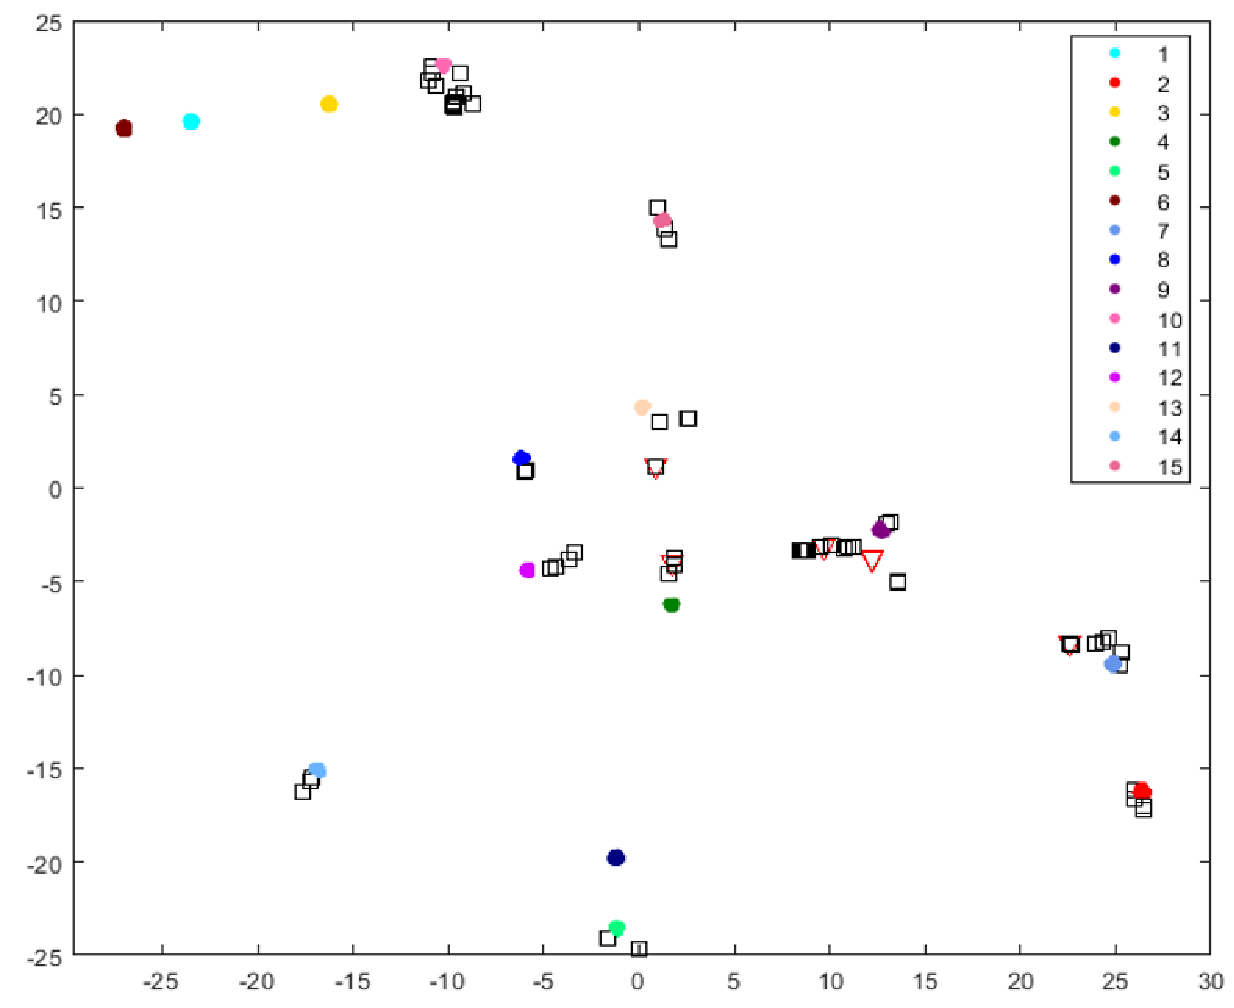
\includegraphics[width=\textwidth]{Figures/2DMvIDDA/Fig7.pdf}
    \caption{MvIDA}
  \end{subfigure}  
  \begin{subfigure}[h]{0.45\textwidth}
    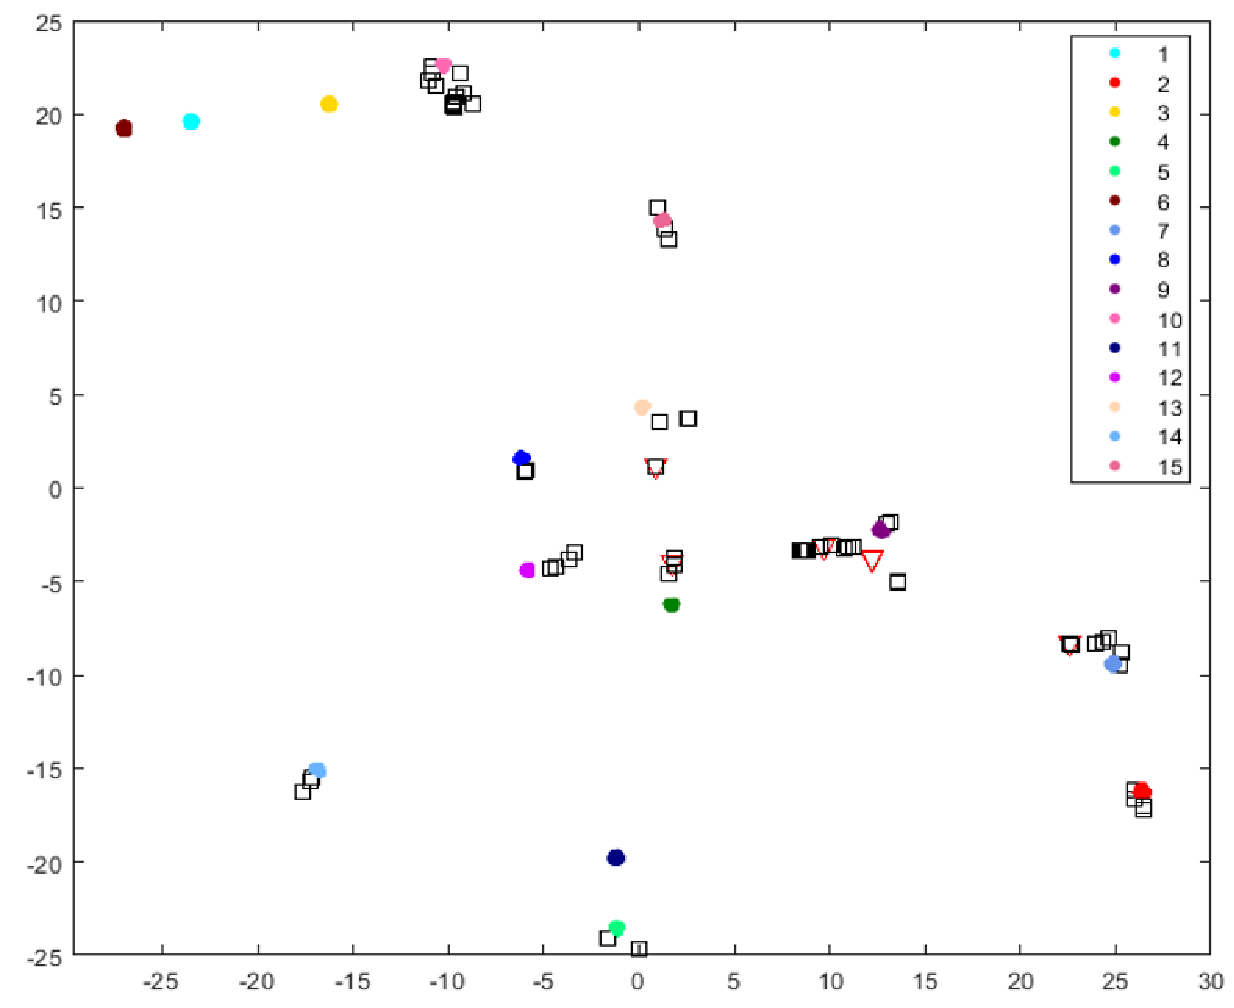
\includegraphics[width=\textwidth]{Figures/2DMvIDDA/Fig8.pdf}
    \caption{MvDA}
  \end{subfigure}  

  \begin{subfigure}[h]{0.45\textwidth}
    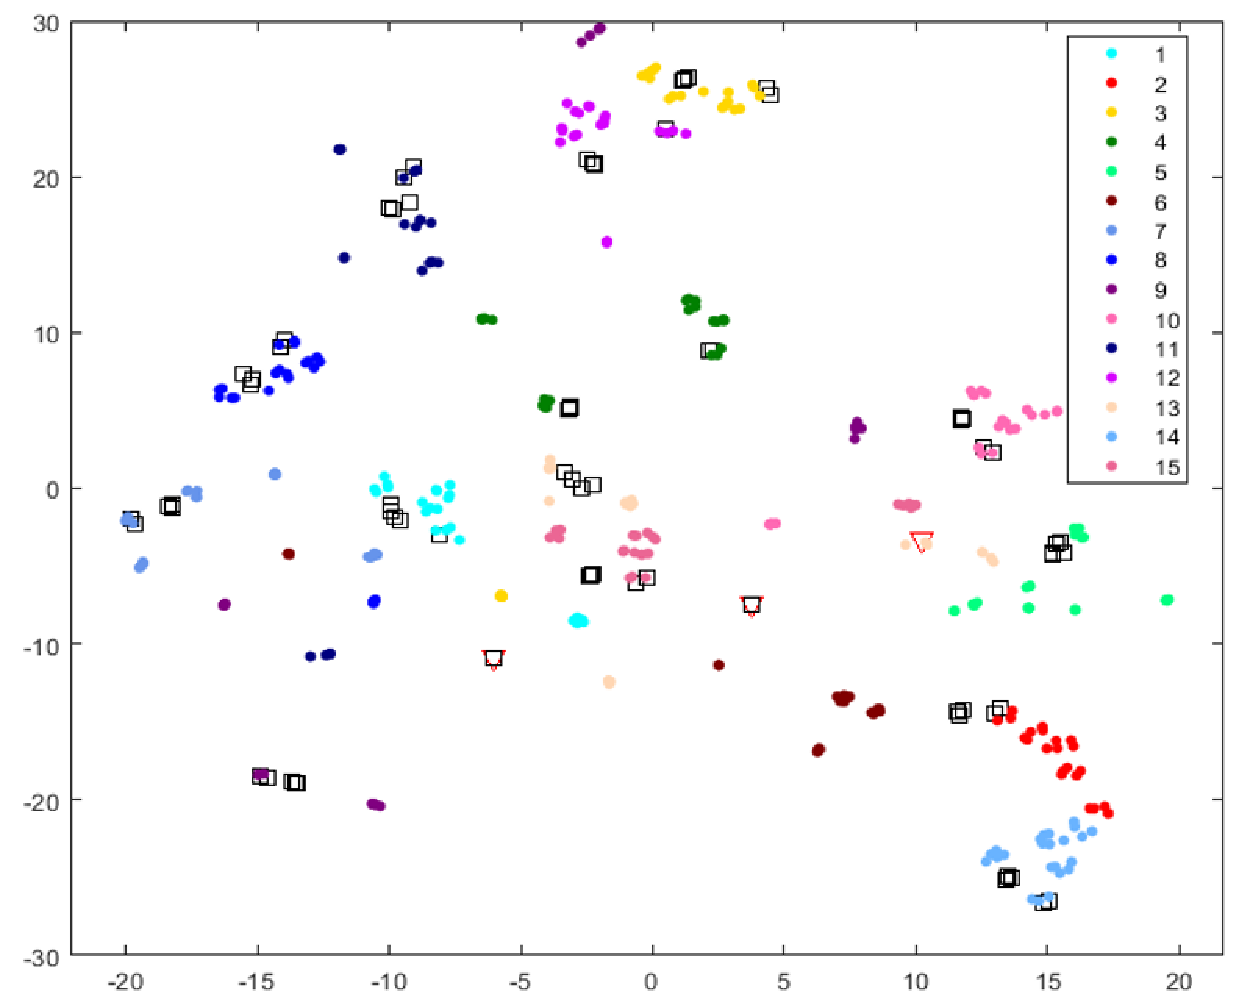
\includegraphics[width=\textwidth]{Figures/2DMvIDDA/Fig9.pdf}
    \caption{2DLDA}
  \end{subfigure}
  \begin{subfigure}[h]{0.45\textwidth}
    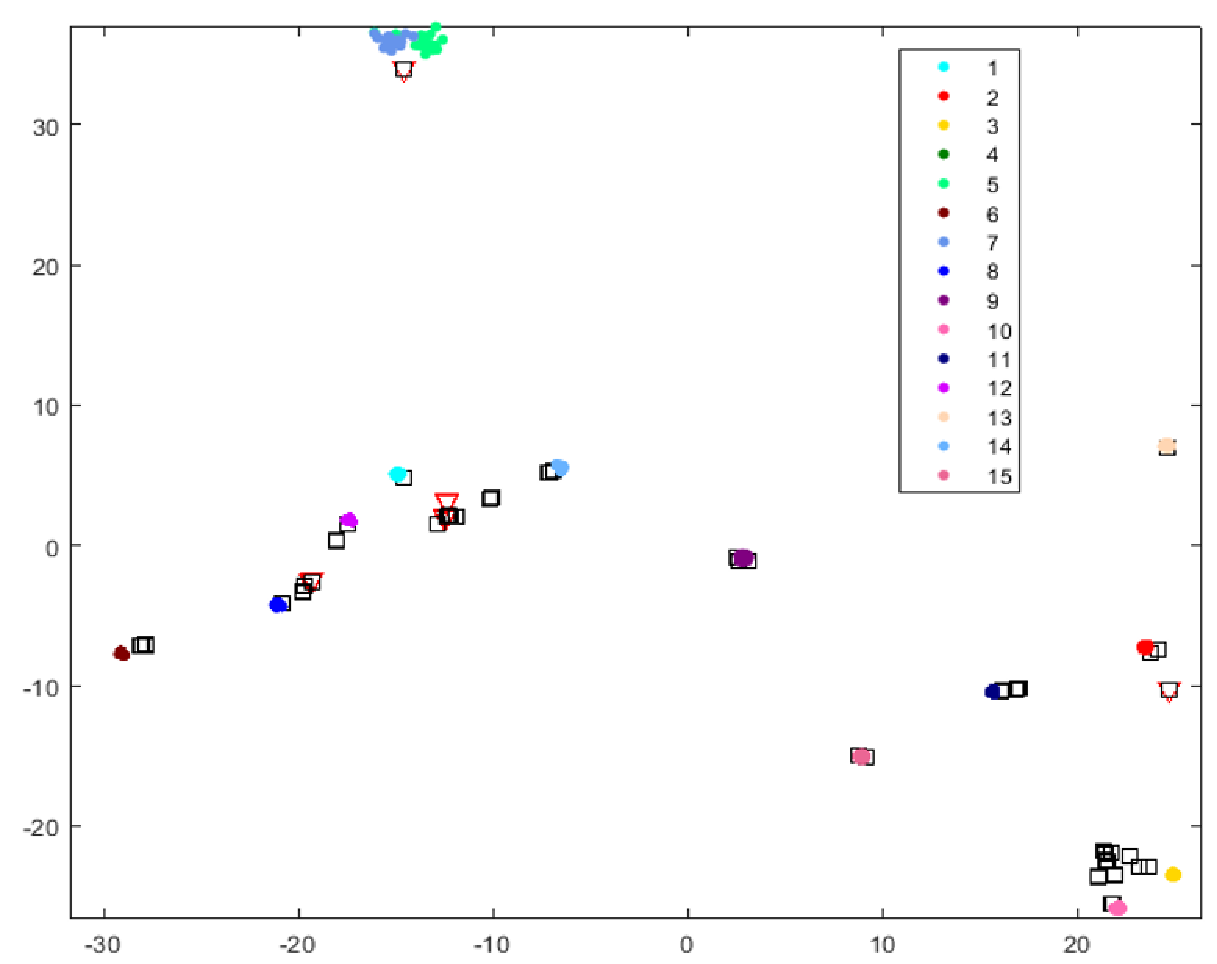
\includegraphics[width=\textwidth]{Figures/2DMvIDDA/Fig10.pdf}
    \caption{ILDA}
  \end{subfigure}
  
\caption{Visualization of Classification on MSSpoof Dataset: (i) Training data samples are denoted with different colored dots for different classes. (ii) Correctly classified test data samples are denoted with black squares. (iii) Misclassified test data samples are denoted with red triangles.}
\label{fig:2DMvIDDA_Res_VisRS}
\end{figure}
\clearpage

\noindent
Unlike the batch methods, it does not need to store the whole dataset. 2DMvDA and 2DLDA too benefit from the use of 2D form. However, these are batch methods and they need to store all data samples and the model. So, the demand for storage increases with the number of data samples. MvIDA and ILDA are incremental methods and do not store old data samples. However, as they use the vectorized format, the size of scatter matrices increases, leading to more memory requirements. MvDA has the largest memory requirements as it is neither an incremental method nor a 2D method. Note that the memory requirements in Table \ref{tab:2DMvIDDA_Res_All_RS} are in MBs.

The time records for the incremental methods consist of the time taken for updating the four entities, namely- the number of data sample, the means, the within-class scatter and the between-class scatter. Similarly, the time records for the batch methods consist of the time taken for recomputing these four entities. We have not considered the time taken for the computation of the projection vectors, as this step is common for both types the methods. The reason for the lesser time requirements of 2DMvIDDA is the same as that for the memory requirements. (i) The 2D form leads to smaller scatter matrices which further leads to less computation time, and (ii) due to the incremental nature of the method, it only requires to \textit{update} the model instead of \textit{retraining} like other batch methods. 2DMvDA and 2DLDA require more time because of their non-incremental nature. However, they need less time than the 1D methods as they operate on smaller scatter matrices. MvIDA and ILDA benefit from the incremental nature, but they need more time because of the larger scatter matrices. Like memory requirements, MvDA is most expensive (except for ILDA) in terms of training time too, as it is a non-incremental 1D method. The reason for ILDA's need for more training time is machine-dependent rather than due to the algorithm itself. As ILDA is a 1D single-view method, the vectorized views are all concatenated and used as the input. In contrast, MvDA and MvIDA use multi-dimensional matrices, which improves their performance even though the total matrix size is the same for these three methods.

The difference between the time and memory requirements of 1D batch and 1D incremental methods is not as much as in the case of 2D methods because the data sample count is significantly less than the number of dimensions. The difference will be more pronounced when the number of data samples is increased.

Figure \ref{fig:2DMvIDDA_Res_VisRS} presents the classification results of these methods on the MSSpoof dataset plotted using t-SNE. The different colored dots represent the training data samples from different classes. The correctly classified test data samples are denoted with black squares, and the incorrectly classified data samples are denoted with red triangles. We can see that the subspace constructed by 2DMvIDDA, 2DMvDA, and 2DLDA is better at discriminating between different classes than that constructed by the 1D methods. Also, The 1D multi-view methods (MvIDA and MvDA) have constructed a better subspace than the 1D single-view method ILDA. This difference in the subspace construction leads to the difference in the classification performance of these methods.
\end{itemize}





\subsubsection{Comparison on the Original Datasets}
\label{ssubs:2DMvIDDA_Orig}
\begin{itemize}
\item \textbf{RQ3 :}
How is this method advantageous than other discriminant analysis-based methods?


\begin{table}[t]
	\centering
	\caption{Comparison of 2DMvIDDA with other 2D methods on the original datasets. Table also lists estimated memory requirements of MvIDA.}
	\label{tab:2DMvIDDA_Res_All_Orig}
	\begin{tabular}{l l r r} \hline
		
		 &  & \textbf{Memory} & \textbf{Training Time} \\
		\textbf{Dataset} & \textbf{Method} & \textbf{(GBs)} & \textbf{(seconds)} \\ \hline
		 
		       & \textbf{2DMvIDDA} & \textbf{1.29} & \textbf{151.19} \\ 
		IMPART & 2DMvDA   & 5.44 & 356.59 \\ 
			   & 2DLDA    & 5.44 & 3094.38 \\
		       & MvIDA    & 1601800 & - \\  \hline
		       
		       & \textbf{2DMvIDDA} & \textbf{0.38} & \textbf{14.07} \\ 
	   MSSpoof & 2DMvDA   & 7.61 & 126.54 \\ 
			   & 2DLDA    & 7.61 & 1686.57 \\
		       & MvIDA    & 102400 & - \\  \hline
		       
		       & \textbf{2DMvIDDA} & \textbf{0.50} & \textbf{10.46} \\ 
		Stereo & 2DMvDA   & 3.94 & 44.90 \\ 
			   & 2DLDA    & 3.94 & 598.85 \\
		       & MvIDA    & 5625 & - \\  \hline
		       
		       & \textbf{2DMvIDDA} & \textbf{0.02} & \textbf{0.41} \\ 
		ORL    & 2DMvDA   & 0.18 & 2.77 \\ 
			   & 2DLDA    & 0.18 & 11.42 \\
		       & MvIDA    & 15.2 & - \\  \hline
	\end{tabular}
\end{table}

\item \textbf{Experiment :}
We train classifiers on the original datasets using only the 2D methods and record their time and memory requirements. Here, the time records for 2DMvIDDA consist of the time taken for updating the four entities, namely- the number of data sample, the means, the within-class scatter and the between-class scatter. Similarly, the time records for 2DMvDA and 2DLDA consist of the time taken for recomputing these four entities. We have not considered the time taken for the computation of the projection vectors, as this step is common for all the methods. To give an idea of the reduction in memory requirements due to the use of 2D data, we also estimated the memory requirements of MvIDA, which requires the least memory among the three 1D methods. Note that the memory requirements are in GBs.

\item \textbf{Discussion :}
Table \ref{tab:2DMvIDDA_Res_All_Orig} lists the training time and memory usage of these 2D methods. We see the same trends with the original datasets as with the rescaled ones. Even among the 2D methods, 2DMvIDDA requires much less memory than the other two methods. However, the main aim here is to show how little are the memory requirements of 2DMvIDDA compared to 1D methods, which is evident from the huge memory requirements of MvIDA. As 1D methods use the vectorized form of input images, the size of scatter matrices increases drastically. In the IMPART dataset, the images are of size $1920 \times 1080$, so scatter matrices computed by the 1D methods will be of size $10368000 \times 10368000$, whereas those computed by the 2D methods are of size $9600 \times 9600$ only. This reduction in the size of scatter matrices saves enormous amounts of memory and training time. ILDA also requires the same amount of memory as MvIDA as it is also a 1D incremental method. Being a batch method, MvDA needs even more memory to store all the historical data.
\end{itemize}














\section{Summary}
\label{sec:2DMvIDDA_conc}
We have presented an incremental-decremental method for 2D multi-view data in this chapter. This method enables the use of the original 2D form of the data to capture the spatial features and multiple views to gather contrasting information. The proposed method does not need to store historical data. It incrementally learns a model by taking only the old model and the data samples to be added. It also decrementally unlearns existing data samples, using the existing model and the data samples to be deleted. 2DMvIDDA is also presented as the generalized form of other discriminant analysis-based methods, namely- 2DMvDA, MvIDA, MvDA, 2DLDA, and ILDA. The formulations of these methods can be obtained from the formulations or a part of the formulations of 2DMvIDDA.

We show that being a scalable method for 2D multi-view data, 2DMvIDDA constructs a better discriminant subspace with significantly less time and memory. This subspace constructed by 2DMvIDDA is the same as that of batch 2DMvDA. 2DMvIDDA also handles data samples from previously unseen classes and is order-invariant.% This work is submitted for peer-review to IEEE Transactions on Cybernetics.

The next chapter presents an incremental-decremental method for multi-view data that can add or remove views from a trained model. This method is also based on discriminant analysis.

\chapterend
\cleardoublepage